%% ---------------- SSHD CONFIGURATION ----------------
\subsection{SSH configurations}
\label{ss:SSHConfiguration}
By default the SSH service are listening on $0.0.0.0$, meaning all interfaces, as seen in the red marked two lines in figure \ref{fig:SSHMngNetwork}.
To achieve the objective regarding minimizing noise traffic to the scanning network interface, the SSH service used for task management must be set to listen to the correct network interface. The usage of SSH on the scanning network interface are not relevant and are therefore strictly limited to the management interface.
The listen address parameter in the SSHd configuration file needs to be changed to the IP address for the management network interface, as seen in listing \ref{lst:SSHDConfiguration}. This parameter change is conducted on each worker through opening the virtual machine in VMware Workstation. The $root$ user must conduct this, since the SSHd configuration file is a file owned by root.
The IP address in line number 2 in listing \ref{lst:SSHDConfiguration} must be changed accordingly to the IP address assigned to the management network interface on the given worker host.

\begin{listing}[!ht]
\caption{Limiting SSH to listen only to the management NIC}
\label{lst:SSHDConfiguration}
\begin{minted}[linenos]{apacheconf}
# Changed parameters from default in file /etc/ssh/sshd_config
ListenAddress 194.100.10.110
\end{minted}
\end{listing}

After this change is done, the SSH service must be restarted.
This must be done by elevating the privileges to $root$ and execute the command in listing \ref{lst:RestartSSHserver}.

\begin{listing}[!ht]
\caption{Restart SSH server}
\label{lst:RestartSSHserver}
\begin{minted}{Bash}
systemctl restart ssh
\end{minted}
\end{listing}

After the SSH server are restarted, the listen address must be validated.
This could be done by executing the command in listing \ref{lst:VerifySSHListening}, and the result of this command is shown in figure \ref{fig:SSHMngNetwork}.
\begin{listing}[!ht]
\caption{List of listening services}
\label{lst:VerifySSHListening}
\begin{minted}{Bash}
ss -lntu
\end{minted}
\end{listing}

\begin{figure}[htbp]
\centerline{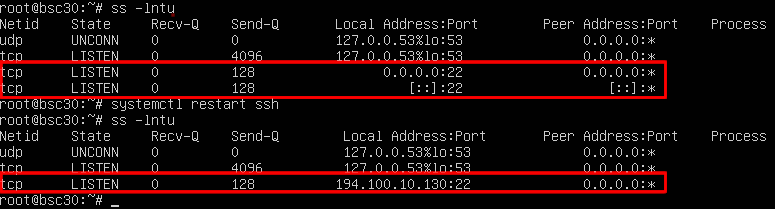
\includegraphics[scale=0.55]{images/misc/SSH-Verified.png}}
\caption{Verifying SSH configuration ListenAddress for management network.}
\label{fig:SSHMngNetwork}
\end{figure}

The last red marked line in figure \ref{fig:SSHMngNetwork} shows that the server only listens to incoming traffic on port 22 when the address is $194.100.10.130$. This means the SSH listening address is verified to only accept incoming connections on the mentioned address.


Furthermore, the key exchange between scanner and worker must be configured.
As a first-time procedure, the key generation for the scanner host needs to be conducted in order to achieve automatic login to a worker without a password prompt.
The command in listing \ref{lst:SSHKeyGeneration} is executed on the scanner host to generate a key pair with both private and public keys.


\begin{listing}[!ht]
\caption{SSH key generation}
\label{lst:SSHKeyGeneration}
\begin{minted}{Bash}
ssh-keygen -t rsa
\end{minted}
\end{listing}


When the key pair is generated, a simple SSH client configuration needs to be implemented in order to achieve automatic login through SSH without receiving a password prompt.
This configuration checks if the worker's hostname matches the criteria $bsc*-mng$, shown in line 2 in listing \ref{lst:SSHClientConfiguration}. In case of a match of the criteria, the configuration defines which default usernames are used to successfully connect to the worker host, shown in line 3 in listing \ref{lst:SSHClientConfiguration}. Also, the given private key to use for the connection is defined in line 4 in listing \ref{lst:SSHClientConfiguration}.

The configuration in listing \ref{lst:SSHClientConfiguration} must be implemented to the file referred to in line 1 on the scanner host to achieve this.

\begin{listing}[!ht]
\caption{SSH client configuration for scanner host}
\label{lst:SSHClientConfiguration}
\begin{minted}[linenos]{apacheconf}
# Implement the following lines to the file /root/.ssh/config
Host bsc*-mng
    User bscadm
    IdentityFile ~/.ssh/id_rsa
\end{minted}
\end{listing}

When these settings are implemented, the public key needs to be authorized on the worker host.
This is step two of the process of enabling authorization using a public key instead of a password prompt.
\begin{listing}[!ht]
\caption{SSH key authorization on worker host}
\label{lst:SSHKeyAuthorization}
\begin{minted}[linenos]{Bash}
ssh-copy-id -i ~/.ssh/id_rsa bscadm@bsc30-mng
ssh bsc30-mng
\end{minted}
\end{listing}

The command in line 1 in listing \ref{lst:SSHKeyAuthorization} adds the key to the authorized keys list in the home directory for the user $bscadm$, as defined in line 3 in listing \ref{lst:SSHClientConfiguration}.
Secondly, in line 2 in listing \ref{lst:SSHKeyAuthorization}, the connection is tested.
The first time logging in on this worker would trigger a prompt for key authorization, which must be accepted before continuing.
From this point forward, the ability to automatically log in to a worker using public-key authorization is enabled.



%% ---------------- /SSHD CONFIGURATION ----------------